\chapter{HPoint хэрэгжүүлэлт}
\section{ER диаграм}

Хэрэглэгч бүр өөрийн гэсэн оноотой байх бөгөөд найзаа урьснаар өөртөө болон найздаа оноо цуглуулж системийг ашиглах юм. Хэрэглэгчийн оноог PointTrans-тай сар бүр тулгаж, ямар нэгэн зөрүү үүсээгүйг баталгаажуулна.
\begin{figure}
\centering
\caption{HPoint Entity relationship диаграм}
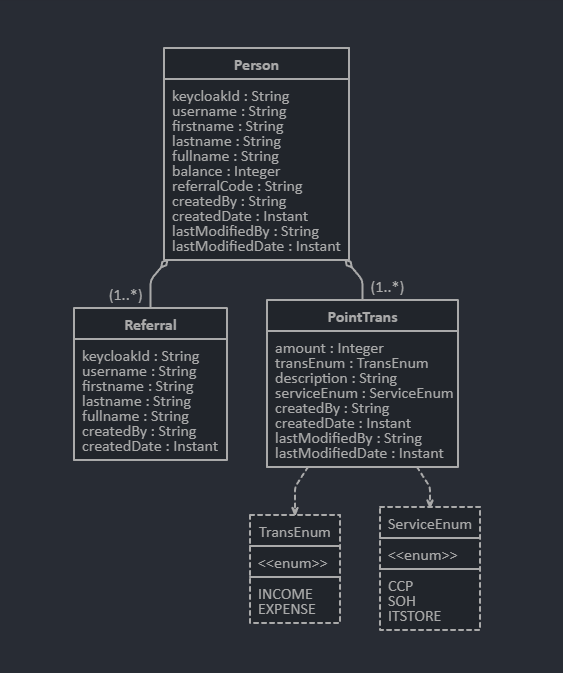
\includegraphics{imgs/erd.png}
\end{figure}

\section{Хэрэглэгчийн интерфейс}

\begin{figure}[h]
  \centering
  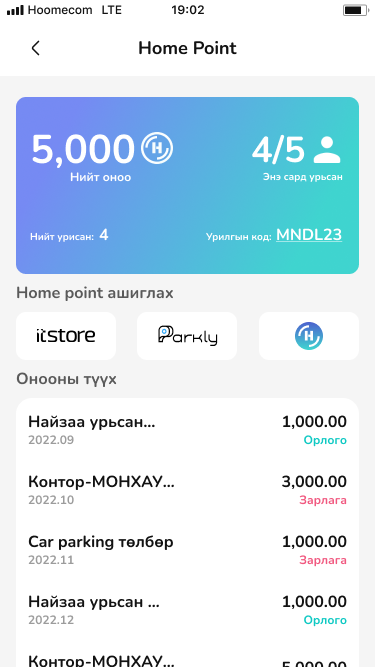
\includegraphics[width=.3\textwidth]{imgs/hpoint.png}
  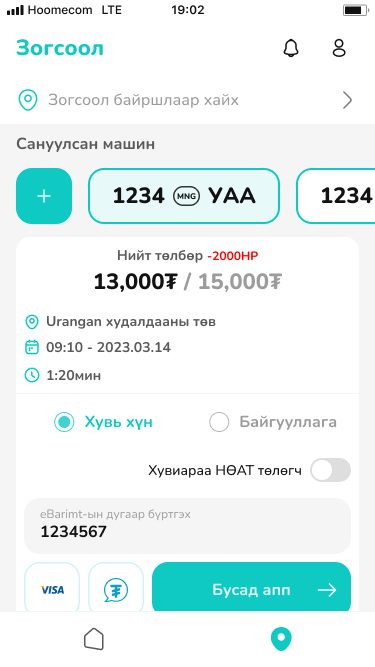
\includegraphics[width=.3\textwidth]{imgs/hpoint-park.png}
  \caption{HPoint нүүр болон төлбөр төлөхөд ашиглалт}
\end{figure}

\begin{lstlisting}[language=Java, frame=single, caption=ITStore нэвтрэх нүүр]
  Container(
    width: double.infinity,
    height: 50,
    decoration: BoxDecoration(
      color: Colors.black,
      borderRadius: BorderRadius.circular(8),
    ),
    child: InkWell(
      onTap: () {
        // ... Auth logic here
      },
      child: Row(
        mainAxisAlignment: MainAxisAlignment.center,
        children: [
          Text(
            'Login',
            style: TextStyle(
                color: Colors.white,
                fontSize: 18,
                fontWeight: FontWeight.w600),
          ),
          Icon(Icons.person, color: Colors.white),
        ],
      ),
    ),
  )
\end{lstlisting}

\begin{lstlisting}[language=Java, frame=single, caption=HPoint нүүр]
BlocBuilder<HPointBloc, HPointState>(
  builder: (context, state) => Container(
      constraints: const BoxConstraints.expand(),
      child: Column(
        children: [
          HoomePointJumbotron(required point: state.point, state.redeemCde),
          PointProvidersScreen(tabController: widget.tabController),
          PointTransactionScreen(),
        ],)),)
\end{lstlisting}